\chapter{Intro and Basics}
\section{Class notes} 
\includepdf[pages={5-9}]{sources/polyEDP-M1-main.pdf}
\section{Techniques : Change of Variables}
\label{sec:Techniques : Change of Variables}
\subsection{Change of Variables for ODE's}
\label{subsec:Change of Variables for ODE's}
We can transform a DE into a easier problem using this method. For instance, consider the
following problem 
\begin{exmp}[Change of Variables]
We have the problem 
\[
y' = F\left( \frac{ y }{ x } \right)    
\]. Since this is homogenous we can rewrite the equation in the form of 
\[
v(x) = \frac{ y }{ x } \implies y = xv  
\]
Using the product rule we get 
\[
y' = v + xv' 
\] 
Using the substitution this gives us 
\begin{align*}
    v + xv' &= F(v) \\ 
    xv' &= F(v) - v \quad \implies \quad \frac{ dv  }{ F(v) - v } = \frac{ d }{ x }   \\ 
\end{align*}
Which is seperable.
\end{exmp}

\begin{exmp}[Change of Variables]
    Another problem is 
    \[
    y' = G\left( ax + by\right) 
    \] which can be solved with 
    \[
    u = ax + by \implies u' = a + by' 
    \]
    which gives 
    \[
        u' = a + G(u) \implies \frac{ du  }{ a + bG(u) } = dx
    \]
\end{exmp}
\subsection{Change of Variables for PDE}
\label{subsec:Change of Variables for PDE}
\begin{exmp}[Change Of Variables]
    Consider the function 
    \begin{equation}
        2 \frac{ dz }{ dx } - \frac{ dz }{ dy } = 0, \qquad \text{ with } z = f(x+2y)
        \label{eq:pde_cof_ex1}
    \end{equation}
    Let $ u = x + 2y $ then we can compute the derivatives using the chain rule. 
    \begin{align*}
        \frac{ \partial f }{ \partial x } &= \left( \frac{ \partial f }{ \partial u }
        \right) \left( \frac{ \partial u }{ \partial x } \right) = f'(u)(1) = f'(u) \\
        \frac{ \partial f }{ \partial y }  &= \left( \frac{ \partial f }{ \partial u }
        \right) \left( \frac{ \partial u }{ \partial y } \right) = 2f'(u) \\ 
    \end{align*}
   Putting those into the equation we get 
   \[
       2f'(u) - 2f'(u) = 0
   \] 
   Using the same function. We can also make the change of variables using $ t = x + 2y $
   and $ s = x $. 
   Taking the derivatives we get 
   \begin{align*}
       \frac{ \partial z }{ \partial x }  &= \frac{ \partial z }{ \partial t } \frac{
       \partial t }{ \partial x } + \frac{ \partial z }{ \partial s } \frac{ \partial s }{
   \partial x} = \frac{ \partial z }{ \partial t } + \frac{ \partial z }{ \partial s }  \\ 
   \frac{ \partial z }{ \partial y }  &= \frac{ \partial z }{ \partial t } \frac{ \partial
   t}{ \partial y } + \frac{ \partial z }{ \partial s } \frac{ \partial s }{ \partial y }
   = 2 \frac{ \partial z }{ \partial t } 
   \end{align*}
   Putting those two into the equations gives us 
   \[
     \frac{ \partial z }{ \partial s } = 0
 \] which shows that $ z $ does not depend on s, thus, any function of the form $ z = f(t)
 $ satisfies the equation. 
\end{exmp}

\begin{exmp}[Change of Variables : 2nd Order PDE]
    Find the formula for $ \frac{ \partial ^2 z }{ \partial r^2 }, \frac{ \partial ^2 z }{
    \partial \theta ^2} , \frac{ \partial ^2 z }{ \partial r \partial \theta  }   $ if $ z
    = f(x,y) $ and $ x = r\cos \theta  $ and $ y = r\sin\theta $.
    $ \\ $
Let $ \xi = f(x,y) $ with $ x = r\cos \theta $ and $ y = r\sin\theta  $ The chain rule
gives us : 
    \begin{align*}
        \frac{ \partial \xi }{ \partial r } &= \frac{ \partial f }{ \partial x } \frac{
        \partial x }{ \partial r } + \frac{ \partial f }{ \partial y } \frac{ \partial y
    }{ \partial r } \\
     &= \frac{ \partial f }{ \partial x } \cos \theta + \frac{ \partial f }{ \partial y }
     \sin\theta \\      
      &\text{ and }  \\ 
      \left( \frac{ \partial  }{ \partial r  } \right) \left( \frac{ \partial \xi  }{
    \partial r } \right)  &=  \frac{ \partial  }{ \partial x } \left( \frac{ \partial \xi
    }{ \partial r } \right) \left( \frac{ \partial x }{ \partial r } \right) + \frac{
\partial  }{ \partial y } \left( \frac{ \partial \xi  }{ \partial r } \right) \left(
\frac{ \partial y }{ \partial r } \right) \\
                          &= \left( \frac{ \partial ^2 f }{ \partial x^2 } \cos\theta +
                          \frac{ \partial ^2 f }{ \partial y \partial x} \sin\theta
                      \right)\cos\theta + \left( \frac{ \partial ^2 f }{ \partial x
                  \partial y } + \frac{ \partial ^2 f }{ \partial y^2 } \sin\theta \right)
                  \sin\theta \\
                          &= \cos^2\theta f_{xx} + 2f_{xy}\cos\theta\sin\theta +
                          \sin^2\theta f_{yy}  \\ 
    \end{align*}
    
\end{exmp}

The difficult with these is using the chain rule for higher order derivatives. 

\subsection{Chain Rule}
\label{subsec:Chain Rule}
We begin with the chain rule for single variable functions. 
\begin{ftheo}[Chain Rule Single Variable]
    \[
        \left( f \circ g\right) ' (x) = f'(g(x) ) g'(x) 
    \]
    \label{th:Chain Rule Single Variable}
\end{ftheo}
Thus, for a second order derivative we have 
\[
    \left( f\circ g\right) ''(x) = \frac{ d }{ dx } \left[ f'(g(x) ) g'(x)  \right]
    = f''(g(x) ) g'(x) g'(x) + f'(g(x) ) g''(x)     
\]
\[
    = f''(g(x) ) \left[ g'(x) \right] ^2 + f'(g(x) ) g''(x) 
\]
Or, using Leibniz notation : 
\[
    \frac{ d^2 f }{ dx^2 } \left( g(x) \right) \left[ \frac{ dg }{ dx } \right] ^2 +
    \frac{ df }{ dx } \left( g(x) \right) \frac{ d^2g }{ dx^2 } 
\]
\begin{ftheo}[Chain Rule for Multivariable Functions]
    \[
    \frac{ \partial f }{ \partial r } = \frac{ \partial f }{ \partial x } \frac{ \partial
    x}{ \partial r } + \frac{ \partial f }{ \partial y } \frac{ \partial y }{ \partial r } 
    \]
    \label{th:Chain Rule for Multivariable Functions}
\end{ftheo}
We can achieve a second order derivative using this rule. 
\[
    \frac{ \partial ^2 f }{ \partial r^2 } = \frac{ \partial  }{ \partial r } \left[
    \frac{ \partial f }{ \partial x } \frac{ \partial x }{ \partial r } \right] + \frac{
    \partial  }{ \partial r } \left[ \frac{ \partial f }{ \partial y } \frac{ \partial y
}{ \partial r } \right]
\]
We first investigate the first term. We need to use the chain rule for $ \frac{ \partial f
}{ \partial x }  $. 
\[
    \frac{ \partial  }{ \partial r } \left[ \frac{ \partial f }{ \partial x } \right] = 
    \frac{ \partial  }{ \partial x } \left( \frac{ \partial f }{ \partial x }
        \frac{ \partial x }{ \partial r }\right) + \frac{ \partial  }{ \partial x } \left(\frac{
\partial f }{ \partial y } \frac{ \partial y }{ \partial r } \right)
\]
\[
 = \frac{ \partial ^2 f  }{ \partial x^2  } \frac{ \partial x }{ \partial r } + \frac{
\partial ^2 f }{ \partial x \partial y } \frac{ \partial y }{ \partial r } 
\]
Thus, 
\begin{align*}
    \frac{ \partial  }{ \partial r } \left[ \frac{ \partial f }{ \partial x }\right] \frac{ \partial x
    }{ \partial r } &= \left( \frac{ \partial ^2 f  }{ \partial x^2  } \frac{ \partial x }{ \partial r } + \frac{ \partial ^2 f }{ \partial x \partial y } \frac{ \partial y }{ \partial r } 
    \right) \frac{ \partial x }{ \partial r } + \frac{ \partial f }{ \partial x } \frac{
\partial ^2 x }{ \partial r^2 }  \\ 
\end{align*}

The other right hand expression of the original equation is found using the same methods : 
\begin{align*}
    \frac{ \partial  }{ \partial r } \left[ \frac{ \partial f }{ \partial y } \frac{
    \partial y }{ \partial r } \right]  &= \left( \frac{ \partial ^2 f  }{ \partial y^2  } 
    \frac{ \partial x }{ \partial r } + \frac{ \partial ^2 f }{ \partial y \partial x } 
    \frac{ \partial y }{ \partial r } 
    \right) \frac{ \partial r }{ \partial r } + \frac{ \partial f }{ \partial y } \frac{
    \partial ^2 y }{ \partial r^2 } \\ 
\end{align*}









\section{Problem Set 1}
\label{sec:Problems Set 1}
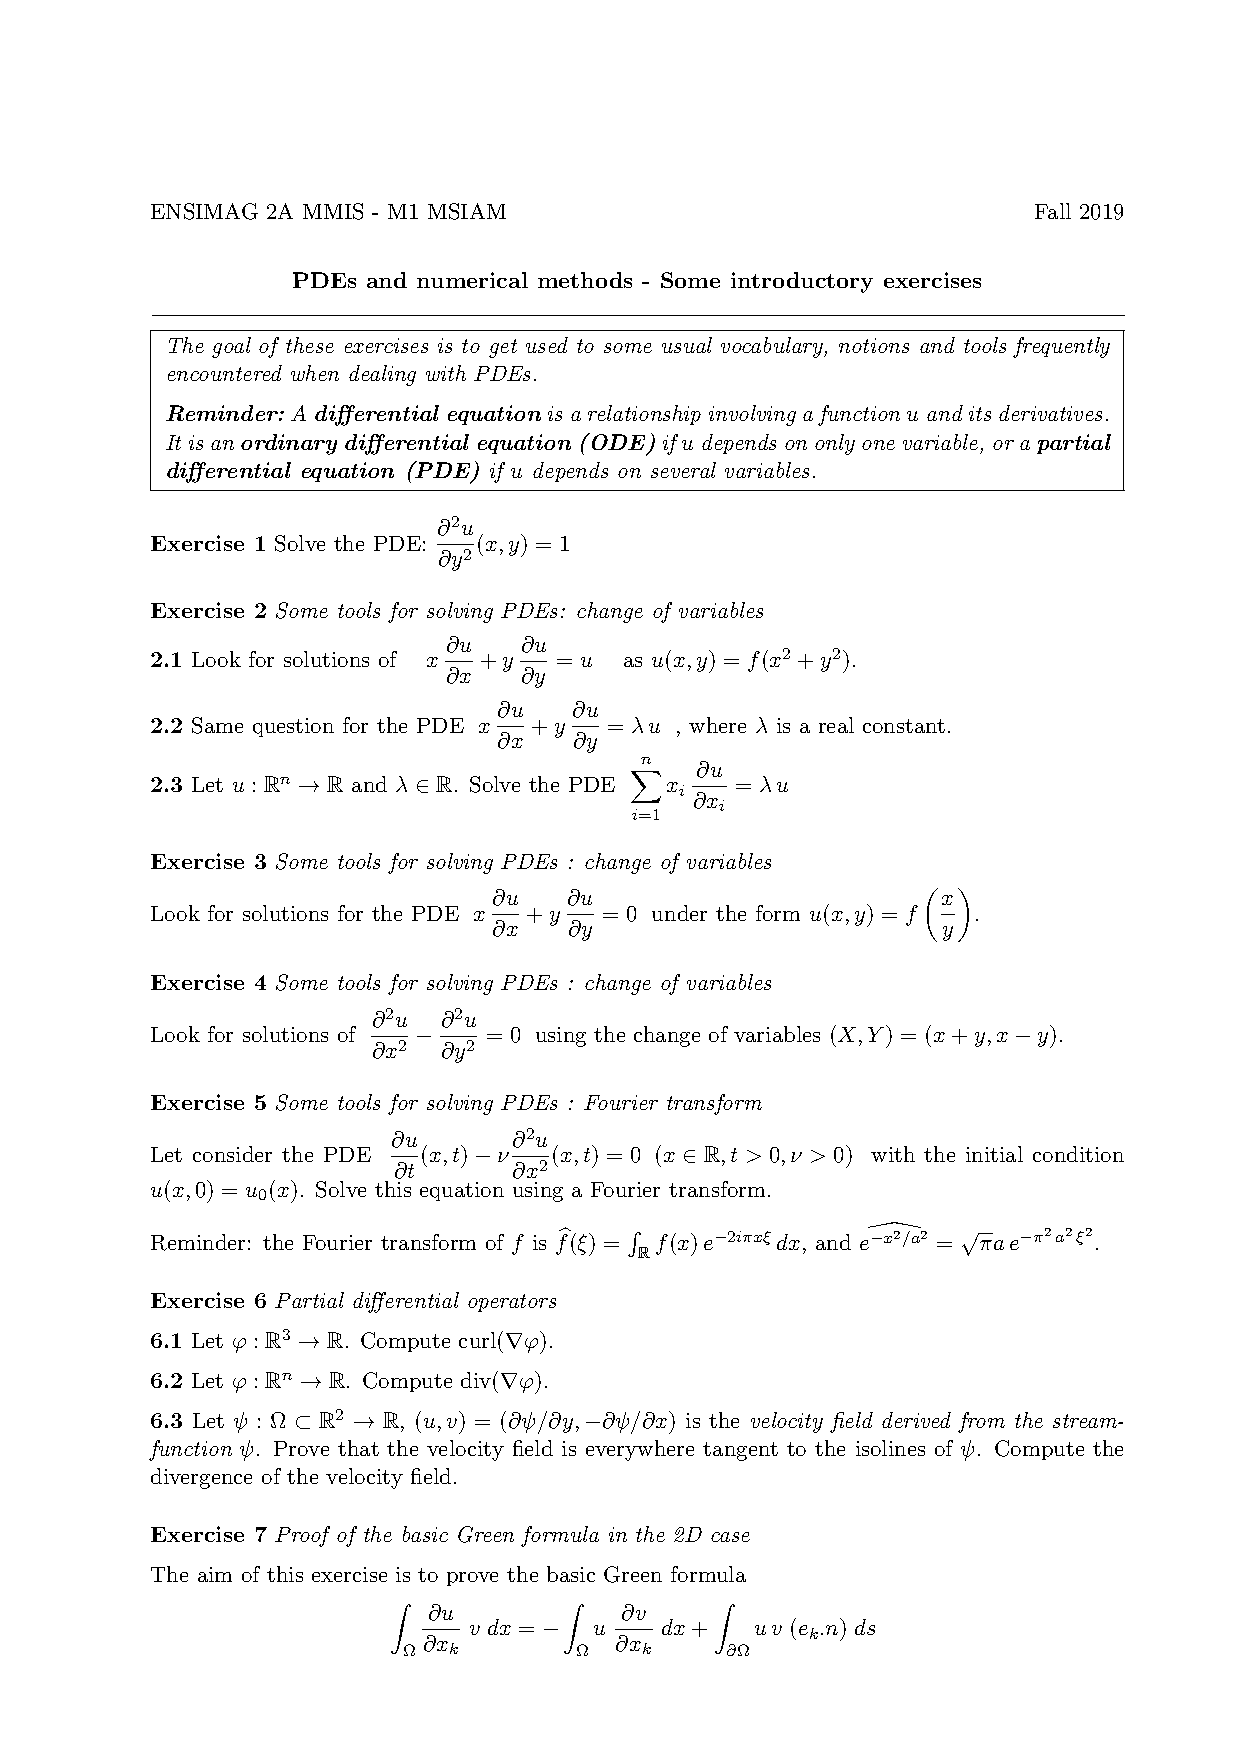
\includepdf[pages=-]{sources/td1.pdf}
\section{Solutions to Problem Set 1}
\label{sec:Solutions to Problem Set 1}
\subsection{Exercise 1}
\label{subsec:Exercise 1}
Solution is simple : 
\begin{align*}
    \frac{ \partial^2 u }{ \partial y^2 } u &= 1 \\ 
    \int\limits_{ }^{ } \frac{ \partial^2 u }{ \partial y^2 } u &= \int\limits_{ }^{ } 1 dy\\ 
    \frac{ \partial u }{ \partial y }  &= y + c(x)  \\ 
    \int\limits_{ }^{ } \frac{ \partial u }{ \partial y } &= \int\limits_{ }^{ } y + c(x)
    dy \\ 
    u &= \frac{ 1 }{ 2 } y^2 + yc(x) + d(x)  \\ 
\end{align*}
\subsection{Exercise 2 : Change of variables }
\label{subsec:Exercise 2 : Change of variables }
\subsubsection{2.1}
Look for solutions of $ x \frac{ \partial u }{ \partial x  } + y \frac{ \partial u  }{
\partial y } = u $ for $ u(x,y) = f(x^2 + y^2) \\ $
First we take the x variable : 
\[
\frac{ \partial u  }{ \partial x } = \frac{ \partial f }{ \partial x } = \left( f'\right)
\left( 2x\right) 
\]
Simlarly for the y variable : 
\[
\frac{ \partial u  }{ \partial y } = \frac{ \partial f }{ \partial y  } = \left( f'
\right) \left( 2y\right) 
\]
Plugging back into the equation : 
\[
2x^2f' + 2y^2f' = f
\]
which can be solved thusly : 
\begin{align*}
    2f' \left( x^2 + y^2 \right) &= f \\
    &\text{Let } x^2 + y^2 = r  \\ 
    \frac{ f' }{ f } &= \frac{ 1 }{ 2 r } \\
    \int\limits_{ }^{ } \frac{ f'  }{ f }  &= \int\limits_{ }^{ } \frac{ 1 }{ 2r }  \\ 
    \ln \left( f\right) &= \frac{ 1 }{ 2 } \ln \left( r\right) + c \\
    f &= e^{\ln(r) / 2 } e^c \\ 
    f &= A\sqrt{r} \quad \text{ where } A = e^c\\ 
\end{align*}
This finally gives us the solution 
\[
    u(x,y) = A\sqrt{x^2 + y^2} \quad A \in \mathbb{R}
\]

\subsubsection{2.2}
Same question for the PDE $ x \frac{ \partial  u }{ \partial x } + y\frac{ \partial u }{
\partial y  }  = \lambda u $ where $ \lambda \in \mathbb{R}  $ and constant.
We begin with the relation 
\[
2rf' = \lambda u 
\]
which gives $ 2rf' = \lambda f $ allowing us to solve. 
\begin{align*}
    2rf'  &= \lambda f \\ 
    \frac{ f' }{ f }  &= \frac{ \lambda  }{ 2r }  \\ 
    \int\limits_{ }^{ } \frac{ f' }{ f } &= \int\limits_{ }^{ } \frac{ \lambda }{ 2r } \\
    \ln\left( f\right)  &= \frac{ \lambda }{ 2 } \ln\left( r\right)  \\ 
    f &= Ar^{ \lambda /  2  } \\ 
\end{align*}
Finally, 
\[
    u(x,y) = A\left( x^2 + y^2 \right) ^{\lambda / 2} 
\]

\subsubsection{2.3}
Let $ u : \mathbb{R} \to \mathbb{R}  $ and $ \lambda \in \mathbb{R}  $. Solve 
\begin{equation}
\sum_{i=1}^{n} x_i \frac{ \partial u }{ \partial x_i } = \lambda u
\label{pr:2.2}
\end{equation}
We first begin with the basic relations 
\[
f(x_1^1 + \cdots + x_n^2) = u(x_1, \cdots , x_n) 
\]
The left hand side of \ref{pr:2.2} elementwise then becomes 
\[
\left( 2x_i^2\right) f'
\] then the entire expression is 
\[
\sum_{i=1}^{n} \left( 2x_i^2 \right) \left( f'\right) = \lambda u
\] then 
\[
\left( 2f'\right) \| x \|^{ 2}_{ } = \lambda f
\] replacing $ \| x \|^{ 2}_{ } = r $ we get 
\begin{align*}
    \frac{ f' }{ f }  &= \frac{ \lambda  }{ 2 } r \\ 
    \ln\left( f\right)  &= \frac{ \lambda  }{ 2 } \ln\left( r\right)  \\ 
    f &= r ^ {\lambda / 2}  \\ 
\end{align*}
So we finally have, 
\[
    \left(  \| x \|^{ 2}_{ } \right) ^ { \lambda / 2} = \|  x \|^{ \lambda }_{ }  
\] 
and our solution is 
\[
u = \| x \|^{ \lambda }_{ } 
\]

\subsubsection{3}
Look for solutions for the PDE $ x \frac{ \partial u }{ \partial x } + y \frac{ \partial u
}{ \partial y } = 0$ under the form $ u(x,y) = f\left( \frac{ x }{ y } \right)  $. 
$ \\ $We first look for x : 
\[
\frac{ \partial f }{ \partial x } = \frac{ f' }{ y }            
\]
for y : 
\[
\frac{ \partial f }{ \partial y } = \frac{ -xf'}{ y^2 } 
\]
Plugging in to the original equation we get
\begin{align*}
    f' \frac{ x }{ y }  - \frac{ x }{ y }f'  &=  0\\ 
    f'\left( \frac{ x }{ y }  - \frac{ x }{ y } \right)  &= 0 \\ 
\end{align*}
which has $ \infty  $ many solutions. 

\subsubsection{Exercise 4}
Look for solutions of $ \frac{ \partial ^2 u  }{ \partial x ^2 } - \frac{ \partial ^2 u }{
\partial y^2 } = 0  $ using $ \left( X, Y\right) = \left( x+y,
x-y\right) . $
\begin{align*}
    \frac{ \partial ^2 f }{ \partial x } - \frac{ \partial^2 f }{ \partial y^2 } = &0\\
\end{align*}
We first compute the left hand side
\begin{align*}
    \frac{ \partial ^2 f  }{ \partial x } &= \frac{ \partial  }{ \partial x } \left(
    \frac{ \partial f }{ \partial x } \right) \\
     &= \frac{ \partial  }{ \partial x } \left( \frac{ \partial f }{ \partial X } \frac{
     \partial X }{ \partial x } + \frac{ \partial f }{ \partial Y } \frac{ \partial Y }{
     \partial x } \right)  \\ 
      &= \frac{ \partial  }{ \partial x } \left( \frac{ \partial f }{ \partial X } +
      \frac{ \partial f }{ \partial Y } \right)  \\ 
\end{align*}

each of these can be a bit tricky. We refer to \ref{th:Chain Rule for Multivariable
Functions} in order to see that 
\begin{align*}
    \frac{ \partial  }{ \partial x } \left( \frac{ \partial f }{ \partial X } \right)  &=
    \frac{ \partial  }{ \partial X } \left( \frac{ \partial f}{ \partial X } \frac{
    \partial X }{ \partial x } + \frac{ \partial f }{ \partial Y } \frac{ \partial Y }{
    \partial x }  \right) \\
     &= \frac{ \partial ^2 f }{ \partial X^2 } \left( 1\right) + \frac{ \partial ^2 f }{
     \partial X \partial Y } \left( 1\right)  \\ 
      &\text{Similarly, for the right hand side}   \\ 
      \frac{ \partial  }{ \partial x } \frac{ \partial f }{ \partial Y }   &= \frac{
      \partial  }{ \partial Y } \left( \frac{ \partial f }{ \partial X } \frac{ \partial x
  }{ \partial x } + \frac{ \partial f }{ \partial Y } \frac{ \partial Y }{ \partial x } \right)  \\
   &= \frac{ \partial ^2 f }{ \partial Y \partial X } \left( 1\right)  + \frac{ \partial^2
   f }{ \partial Y^2 } \left( 1\right)  \\ 
\end{align*}
This leaves us with  
\[
\frac{ \partial ^2 f }{ \partial x^2  } = \frac{ \partial ^2f }{ \partial X^2 } +
\frac{ \partial ^2f }{ \partial X \partial Y } + \frac{ \partial ^2f }{ \partial Y
\partial X } + \frac{ \partial ^2f }{ \partial Y^2 }     
\]
For the second term, 
\begin{align*}
    \frac{ \partial ^2 f }{ \partial y^2  } &= \frac{ \partial  }{ \partial y } \left(
    \frac{ \partial f }{ \partial y } \right) \\
     &= \frac{ \partial  }{ \partial y } \left( \frac{ \partial f }{ \partial X } \frac{
     \partial X }{ \partial x } + \frac{ \partial f }{ \partial Y } \frac{ \partial Y }{
     \partial y } \right)  \\ 
     &= \frac{ \partial  }{ \partial y } \left( \frac{ \partial f }{ \partial X } - \frac{
     \partial f }{ \partial Y } \right)  \\ 
\end{align*}
Thus, 
\begin{align*}
    \frac{ \partial  }{ \partial y } \left( \frac{ \partial f }{ \partial X } \right) &=
    \frac{ \partial  }{ \partial X } \left( \frac{ \partial f }{ \partial X } \frac{
    \partial X }{ \partial y } + \frac{ \partial f }{ \partial Y } \frac{ \partial Y }{
    \partial y } \right) \\
     &= \frac{ \partial  }{ \partial X } \left( \frac{ \partial f }{ \partial X } - \frac{
     \partial f }{ \partial Y }  \right)  \\ 
     &= \frac{ \partial ^2 f }{ \partial X^2 } - \frac{ \partial ^2 f }{ \partial X
     \partial Y }  \\ 
\end{align*}

and, 

\begin{align*}
    \frac{ \partial  }{ \partial y } \left( \frac{ \partial f }{ \partial Y } \right)  &=
    \frac{ \partial  }{ \partial Y } \left( \frac{ \partial f }{ \partial X } \frac{
    \partial X }{ \partial y } + \frac{ \partial f }{ \partial Y } \frac{ \partial Y }{
    \partial y } \right) \\ 
     &= \frac{ \partial  }{ \partial Y } \left( \frac{ \partial f }{ \partial X } - \frac{
     \partial f }{ \partial Y } \right)  \\
      &= \frac{ \partial ^2f }{ \partial Y \partial X } - \frac{ \partial ^2f }{ \partial
      Y^2}  \\ 
\end{align*}

which gives 
\[
\frac{ \partial ^2 f }{ \partial y^2 } =  \frac{ \partial  }{ \partial y } \left( \frac{ \partial f }{ \partial X } \right) - \frac{
\partial  }{ \partial y }\left( \frac{ \partial f }{ \partial Y } \right) = \frac{
\partial ^2f }{ \partial X^2 } - \frac{ \partial ^2 f }{ \partial X \partial Y } - \frac{
\partial ^2 f}{ \partial Y \partial X  } + \frac{ \partial ^2f }{ \partial Y^2 }  
\]
Plugging in to the original equation : 

\[
\frac{ \partial ^2 f }{ \partial x^2  } - \frac{ \partial ^2f }{ \partial y^2 } = 
\frac{ \partial ^2f }{ \partial X^2 } +
\frac{ \partial ^2f }{ \partial X \partial Y } + \frac{ \partial ^2f }{ \partial Y
\partial X } + \frac{ \partial ^2f }{ \partial Y^2 }     
- \left(  \frac{
\partial ^2f }{ \partial X^2 } - \frac{ \partial ^2 f }{ \partial X \partial Y } - \frac{
\partial ^2 f}{ \partial Y \partial X  } + \frac{ \partial ^2f }{ \partial Y^2 }   \right) 
\]
\[
= 0 + 2 \frac{ \partial ^2f }{ \partial X \partial Y } + 2 \frac{ \partial ^2f }{ \partial
Y \partial X} + 0
\]
Assuming mixed partials are equal we get 
\[
\frac{ \partial ^22f }{ \partial X \partial Y } = 0
\]
So we are looking for $ u \in \mathscr{ C } ^2 $ such that the mixed partials are equal to
zero. This gives us the function 
\[ u = F\left( x+y\right) + G\left( x-y\right)  
    \qquad \text{where } F,G \in \mathscr{ C } ^2. 
\]


\subsection{Fourier Transform}
\label{subsec:Fourier Transform}
\begin{equation}
    \frac{ \partial u }{ \partial t } \left( x, t\right) - \nu \frac{ \partial ^2u }{
    \partial x^2 } \left( x,t\right) = 0, \qquad x \in \mathbb{R}, t> 0, \nu > 0 
\end{equation}
With $ u\left( x,0\right) = u_0(x) \\$. 
We want to solve this using the Fourier Transform which we denote using 
\[
    \mathscr{ F } \left( f(x) \right) = \widehat{f}(\xi) = \int\limits_{ \mathbb{R}}^{ }
    f(x) e^{-2i\pi x\xi} \ dx 
\]
Using basic properties of the Fourier Transform we have : 
\[
    \frac{ \partial u }{ \partial t } \widehat{u}(\xi, t) - \nu \left( 2\pi i \xi\right)
    ^2 \widehat{u}(\xi,t) 
\]
\[
    \frac{ \partial u }{ \partial t } \widehat{u}(\xi, t) + \nu4\pi^2\xi^2 \widehat{u}(\xi,t) 
\]
Which gives a seperable equation 
\[
    \int\limits_{ }^{ }  \frac{ du  }{ u } = -\int\limits_{ }^{ } \nu4\pi^2\xi^2 \ dt 
\]
\[
    \widehat{u} = Ae^{-v4\pi^2\xi^2t} \qquad \text{ where } A = e^{cst}
\]
Using initial conditions we have 
\[
    \widehat{u}(\xi, 0) = A = \widehat{u}_0(\xi)
\]
\[
    \widehat{u}(\xi, t) = \widehat{u}_0(\xi)e^{-\nu4\pi^2\xi^2 t}
\]
Using the fact that $ \widehat{e^{-x^2/a}} = \sqrt{\pi} ae^{-\pi^2a^2\xi^2} $, we have : 
\begin{align*}
    \pi^2 a^2 \xi^2  &= \nu 4\pi^2\xi^2 t \\ 
    a^2 &= \nu 4t  \\ 
    a &= 2\sqrt{\nu t}\\
     &\text{ Then, substituting for a }  \\ 
    \mathscr{ F } \left( e _{  }^{ -x^2 / 2\sqrt{\nu t } }\right)  &= 2\sqrt{\pi\nu
    t} e _{  }^{ -\nu4\pi^2  \xi^2 t } \\ 
        \mathscr{ F } \left( \frac{1  }{  2\sqrt{\pi \nu t} } e _{   }^{ -x^2 / 2\sqrt{\nu
        t} }  \right)      &= e _{  }^{ -\nu4\pi^2  \xi^2 t }
\end{align*}
Finally, 
\begin{align*}
    \mathscr{ F } \left( u_0(x)\frac{1  }{  2\sqrt{\pi \nu t} } e _{   }^{ -x^2 / 2\sqrt{\nu
    t} }  \right)      &= u_0(x)e _{  }^{ -\nu4\pi^2  \xi^2 t } 
\end{align*}
\[
u(x,t) &= \frac{ 1 }{ 2\sqrt{\pi\nu t}  } \int\limits_{-\infty}^{\infty} u_0(y) e _{
    }^{ \frac{ -\left( x-y\right) ^2 }{ 4\nu t }  } \ dy \\ 
\]







\subsection{Partial Differential Operators}
\label{subsec:Partial Differential Operators}
\begin{enumerate}
    \item Let $ \varphi : \mathbb{R}^3 \to \mathbb{R} $. Compute curl $ \left( \nabla
        \varphi\right)  $
    \item Let $ \varphi : \mathbb{R}^n \to \mathbb{R} $. Compute div $ \left( \nabla
        \varphi  \right)$
    \item Let $ \psi : \Omega \subset \mathbb{R}^2 \to \mathbb{R} $, $ (u,v) = \left(
        \partial \psi / \partial y, - \partial \psi / \partial x\right)  $
    is the velocitiy field derived from the stream function $ \psi $. Prove that the
    velocity field is everywhere tangent to the isoline of $ \psi $. Compute the
    divergence of the velocity field. 
\end{enumerate}
Using the fact that, for $ \varphi : \mathbb{R}^n \to \mathbb{R}  $ we have that 
\[
            \text{grad } \varphi(\boldsymbol{x}) = \nabla \varphi( \boldsymbol{x} ) = \begin{pmatrix*}
                \frac{ \partial \varphi }{ \partial x_1 }  \\
                 \vdots \\
                 \frac{ \partial \varphi }{ \partial x_n } 
            \end{pmatrix*}
\]


\begin{enumerate}
    \item 
        \begin{align*}
            \text{curl } \varphi(\boldsymbol{x} ) &= \text{curl } \begin{pmatrix*}[r]
                \frac{ \partial \varphi }{ \partial x_1 }   \\[0.5em]
                \frac{ \partial \varphi }{ \partial x_2 }  \\[0.5em]
                 \frac{ \partial \varphi }{ \partial x_3 }  
            \end{pmatrix*}
               \\ 
                &= \begin{pmatrix*}[r]
                    \frac{ \partial ^2 \varphi }{ \partial x_2 \partial x_3 } - \frac{
                    \partial ^2 \varphi }{ \partial x_3 \partial x_2 }   \\[1em] 
                    \frac{ \partial ^2 \varphi }{ \partial x_3 \partial x_1 } - \frac{
                    \partial ^2 \varphi }{ \partial x_1 \partial x_3 }   \\[1em] 
                    \frac{ \partial ^2 \varphi }{ \partial x_1 \partial x_2 } - \frac{
                    \partial ^2 \varphi }{ \partial x_2 \partial x_1 }   \\
                \end{pmatrix*}
                  \\ 
        \end{align*}
    \item   \[\text{div } \varphi(\boldsymbol{x} ) &= \text{curl } \begin{pmatrix*}
                \frac{ \partial \varphi }{ \partial x_1 }   \\[0.5em]
                \vdots  \\[0.5em]
                 \frac{ \partial \varphi }{ \partial x_n }  
            \end{pmatrix*}
        \]
        \[
        = \sum_{i=1}^{n} \frac{ \partial^2 \varphi_i }{ \partial x^2_i } 
        \]
\end{enumerate}

\subsection{Proof of the basic Green Formula in the 2D case}
\label{subsec:Proof of the basic Green Formula in the 2D case}
We want to prove 
\begin{equation}
\int\limits_{\Omega}^{ } \frac{ \partial u }{ \partial x_k } v \ dx = -
\int\limits_{\Omega}^{ } u \frac{ \partial v  }{ \partial  x_k  } \ dx + \int\limits_{
\partial \Omega } uv \left( e_k \cdot n \right) \ ds
\label{eq:general_green_formula}
\end{equation}
where $ e_k $ is the unit vector in direction $ x_k $, in the 2D-case $ \left( \Omega
\subset \mathbb{R} \right)  $.

\begin{figure}[ht]
    \centering
    \incfig{greenonomega}
    \caption{greenOnOmega}
    \label{fig:greenonomega}
\end{figure}

\newpage 
\subsubsection{7.1}
Prove this formula for $ \Omega  $ being the reference triangle (i.e, with nodes $ \left(
0,0\right) , \left( 1,0\right) , \left( 0,1\right)  $). 
\begin{figure}[ht]
    \centering
    \incfig{green-on-t}
    \caption{green on T}
    \label{fig:green-on-t}
\end{figure}
 
The left hand side of \ref{eq:general_green_formula} becomes 
\[
\int\limits_{\Omega}^{ } \frac{ \partial u }{ \partial x_1 } v \ dx_1 dx_2 
\] or 
\begin{align*}
    \int\limits_{T}^{ } \frac{ \partial u }{ \partial x_1 } v\ dx_1dx_2  &= 
    \int\limits_{x_1 = 0}^{1} \left( \int\limits_{x_2 = 0}^{x_2= 1
    - x_1 } \frac{ \partial u }{ \partial x_1 } v \ dx_2\right) dx_1 \\
     &= \int\limits_{x_2 = 0}^{1} \left( \int\limits_{x_1 = 0}^{1 - x_2} \frac{ \partial u
     }{ \partial x_1 } v \ dx_1\right) dx_2 \\ 
\end{align*}
The last formulation has a fixed $ x_2 $ for the inner part of the equation. 

\begin{prop}[]
    \[
        \int\limits_{ \partial \Omega} f \ d\sigma = \sum_{i=1}^{m} \int\limits_{ \partial
        \Omega_i }^{ } f \ d\sigma 
    \]
    That is, each side of the boundary can be analyzed independently for simple
    parametrization, furthermore, the combination of the pieces is that integral of the
    entire boundary. $ \\ $
    We get the following formation due to the defintion of a line integral :  
    \[
        \int\limits_{ \partial \Omega} f \ d\sigma = \int\limits_{0}^{1} f\left(
        \gamma_i(t) \right) \| \gamma'_i(t) \|^{ }_{ } \ dt 
    \]
\end{prop}

Furthermore, we calculate the unit normal for each segment of the triangle. 
\[
\partial T_1 = \begin{pmatrix*}[r]
    0 \\
    0 
\end{pmatrix*}
- \begin{pmatrix*}[r]
     1 \\
     0 
\end{pmatrix*}
 = \begin{pmatrix*}[r]
      -1 \\
      0 
 \end{pmatrix*}
 \text{ which has normal } n_1 = \begin{pmatrix*}[r]
     0  \\
     -1 
 \end{pmatrix*}
 
\] 

\[
\partial T_2 = \begin{pmatrix*}[r]
     1 \\
     0 
\end{pmatrix*}
- \begin{pmatrix*}[r]
    0 \\
    1 
\end{pmatrix*}
= \begin{pmatrix*}[r]
     1 \\
    -1 
\end{pmatrix*}
\text{ which has length } \| \cdot  \|^{ }_{ } = \sqrt{2}
\]
thus, 
\[
\begin{pmatrix*}[r]
     1 \\
     -1 
\end{pmatrix*}
\cdot \begin{pmatrix*}[r]
     1 \\
     1 
\end{pmatrix*}
= 0 , 
\]
 and we divide by the length to ensure the normal has length 1
\[
\partial T_2 = \begin{pmatrix*}[r]
    \frac{ 1 }{ \sqrt{2}} \\[0.5em]
    \frac{ 1 }{ \sqrt{2} }  
\end{pmatrix*}
\]
The last is found simply, 
\[
\partial T_3 = \begin{pmatrix*}[r]
    -1 \\
     0
\end{pmatrix*}
\]
We can now solve for each side. 

\[
    \int\limits_{x_2=0}^{1} \left( - \int\limits_{x_1=0}^{1-x_2} u \frac{ \partial v  }{
    \partial x_1 } \right) \ dx_2 +  \int\limits_{x_2=0}^{1} u\left( 1-x_2, x_2\right)
    v\left( 1-x_2, x_2\right) - u\left( 0,x_2\right) v\left( 0,x_2\right) \ dx_2
\]
\begin{align*}
    \int\limits_{ \partial T}^{ } uvn_1 \ d\sigma &= \int\limits_{ \partial
    T_1}^{ } uv\overbrace{ n_1}^{=0} \ d\sigma + \int\limits_{ \partial T_2 }^{ }
    uv\overbrace{n_1}^{=1/\sqrt{2}} + \int\limits_{ \partial T_3}^{ }
    uv\overbrace{n_1}^{=-1} \ d \sigma \\
     &= \int\limits_{ \partial T_2}^{} uvn_1 \ d\sigma + \int\limits_{ \partial T_3}^{ }
     uvn_1 \ d\sigma   \\ 
\end{align*}
Now, for $ \partial T_2 $ we have the paramaterized line as 
\[
    \gamma_2 (t) = \set{ \left( 1-t, t\right) , t\in [0,1] } \text{ where } \gamma_2'(t) =
    \begin{pmatrix*}[r]
        -1 \\
         1 
    \end{pmatrix*}
    \text{ and } 
    \| \gamma_2' \|^{ }_{ } = \sqrt{2}
\]
Finally, 
\[
    \int\limits_{0}^{1} u\left( 1-t, t\right) v\left( 1-t, t\right) \frac{ 1 }{ \sqrt{2} }
    \sqrt{2} \ dt 
\]
Since $ \gamma_3(t) = \set{ \left( 0, 1-t\right)  }  $ we have 
\[
    \int\limits_{0}^{1} u\left( 0,t\right) v\left( 0,t\right) (-1) \cdot (1) \ dt
\]
and 
\[
\int\limits_{0}^{1} u\left( 1-t, t\right) v\left( 1-t, t\right) -  u\left( 0,t\right) 
v\left( 0,t\right) \ dt
\]

\subsection{Green Formulas}
\label{subsec:Green Formulas}
\begin{enumerate}
    \item \[
            \int\limits_{\Omega}^{ } \text{div}\left( \boldsymbol{E} (\boldsymbol{x})
            \right) \ d\boldsymbol{x} \quad \text{ with } \boldsymbol{E} : \Omega \subset
            \mathbb{R}^n \to \mathbb{R}^n
    \]
First, it should be noted that the div of a function is a scalar, and we take u = 1. Thus, 
\begin{align*}
    \int\limits_{\Omega}^{ } u \text{ div}(\boldsymbol{E}) \ dx &= - \int\limits_{\Omega}^{ }
    \underbrace{\nabla u}_{=0} \cdot \boldsymbol{E} + \int\limits_{ \partial \Omega }^{ } u \left(
\boldsymbol{E} \cdot \boldsymbol{n} \right) \ ds \\
 &= \int\limits_{ \partial \Omega} u \left( \boldsymbol{E} \cdot \boldsymbol{n}  \right) \
 ds\\ 
 &\text{ since } u = 1\\
    \int\limits_{\Omega}^{ } \text{div} \left( \boldsymbol{E} \right) \ dx &= \int\limits_{
 \partial \Omega}^{ } \boldsymbol{E} \cdot \boldsymbol{n} \ ds 
\end{align*}

\item \[
        \int\limits_{\Omega}^{ } \text{div}\left( k(\boldsymbol{x}) \nabla
        u(\boldsymbol{x})   \right) \ d\boldsymbol{x} 
        \quad \text{ with } u : \Omega \subset \mathbb{R}^n\to \mathbb{R}
\]
\begin{align*}
    \int\limits_{\Omega}^{ } \text{div}\left( k(\boldsymbol{x} ) \nabla u(\boldsymbol{x} )
    \right) \ d\boldsymbol{x}   &=  \\ 
\end{align*}

\item 
    \[
    \int\limits_{\Omega}^{} \sum_{i=1}^{n} \alpha_i \frac{ \partial u }{ \partial x_i }
    \frac{ \partial v  }{ \partial x_i } \quad \text{ with } u,v : \Omega \subset
    \mathbb{R}^n \to \mathbb{R} \text{ and } \alpha_i \in \mathbb{R} 
    \]
\end{enumerate}


\subsection{Boundary conditions and well-posedness}
\label{subsec:Boundary conditions and well-posedness}

\subsubsection{9.1}
Let the ODE 
\[
    u''(x) = 0 \text{ in } ]a,b[
\]
Find its solution considering 
\begin{enumerate}[label={(\alph*)}]
    \item Dirichlet Conditions : $ u(a) = \alpha, \ u(b) = \beta $
    \item Neumann conditions : $ u'(a) = \alpha , \ u'(b) = \beta  $
    \item Robin conditions : $ u'(a) + \lambda u(a) = \alpha, \ u'(b) + \lambda u(b) =
        \beta  $ with $ \lambda \neq 0 $
    \item Mixed conditions : $ u'(a) = \alpha $, $ u(b) = \beta $
\end{enumerate}
We begin with the fact that this ODE has the general form of 
\[
    u(x) = Ax + B
\]
\begin{enumerate}[label={(\alph*)}]
    \item This gives us the condition that 
        \[
            u(a) = Aa + B = \alpha \qquad u(b) = Ab + B = \beta 
        \]
        Intuitively, this is well posed because there exists a unique line between two
        points. In terms of a solution we get : 
        \[
            A = \frac{ \beta - \alpha  }{ b - a } \qquad B = \alpha - \frac{ \beta -\alpha
            }{ b-a } (a) 
        \]
    \item Since $ u'(x) = A = \alpha = \beta $ which does not guarantee uniqueness. 
    \item 
        \[
            A + \lambda \left(Aa + B  \right) = \alpha \qquad A + \lambda \left( Ab + B\right)  = \beta 
        \] which gives us 
        \[
            A\left( 1 + \lambda a\right) + \lambda B = \alpha \qquad A\left( 1 + \lambda
            b\right) + \lambda B = \beta 
        \]
        we can test linear dependence via the determinate, which gives 
        \[
        \lambda\left( 1 + \lambda a\right) - \lambda\left( 1 + \lambda B\right) =
        \lambda^2\left( a-b\right) \neq 0
        \]
    \item The last conditions give : 
        \[
        u'(a) = \alpha \implies A = \alpha \qquad \text{ then } u(b) = \alpha b + B
        \implies B = \beta - \alpha b
        \] 
        This solution is unique since it depends on both endpoints. 
\end{enumerate}


\subsubsection{9.2}
Consider 
\begin{equation}
    \triangle u = f \quad \text{ on } \Omega \subset \mathbb{R}^n
    \label{eq:9.2}
\end{equation}
\begin{enumerate}[label={(\alph*)}]
    \item Dirichlet conditions : $ u = g  $ on $ \partial \Omega  $
    \item Neumann conditions : $ \frac{ \partial u }{ \partial n  } = h $ on $ \partial
        \Omega $
    \item Mixed conditions : 
        \[
        u = g \text{ on } \Gamma_0, \quad \frac{ \partial u }{ \partial n  } = h \text{ on
        } \Gamma_1, \text{ where } \Gamma_0 \cup \Gamma_1 = \partial \Omega \text{ and }
        \Gamma_0 \cap \Gamma_1 = \emptyset 
        \]
\end{enumerate}
(a) 
We use the approach of assuming that there can be two solutions which result in a
contradiction. Let $ u_1,u_2 $ be two solutions of $ \triangle u = f \text{ on } \Omega $.
We then have 
\[
    \begin{aligned} 
&\begin{cases} 
    \begin{aligned}
        \triangle u_1 &= f \text{ in } \Omega \qquad \\
        u_1 &= g \text{ on } \partial \Omega 
    \end{aligned}
\end{cases}
&\begin{cases} 
    \begin{aligned}
        \triangle u_2 &= f \text{ in } \Omega \qquad \\
        u_2 &= g \text{ on } \partial \Omega 
    \end{aligned}
\end{cases}
\end{aligned} 
\]
If $ u_1,u_2 $ solutions then $ u = u_1 - u_2  $ is a solution 
\[
\begin{cases}
    \begin{aligned}
        \triangle u &= f - f = 0 \quad &\text{ in } &\Omega   \\ 
        u &= g - g = 0 \quad &\text{ on } &\partial   \Omega   \\ 
    \end{aligned} 
\end{cases}
\]

Using Green's theorem we get : 
\begin{align*}
    \int\limits_{\Omega}^{ } \triangle u v \ dx &= - \int\limits_{\Omega}^{ } \triangle u
    \triangle v \ dx + \int\limits_{ \partial \Omega }^{ } \partial _nuv \ d\sigma \\ 
     &\text{Where } \partial _nu \text{ or } \frac{ \partial u }{ \partial n  } = \nabla
     u\cdot n \text{ or } \sum_{}^{} \frac{ \partial u }{ \partial x_k }   \\ 
      &\text{Can be found in the class slides}  \\ 
      &= \int\limits_{\Omega}^{ } \underbrace{\triangle u}_{=0} v \ dx - \int\limits_{
      \partial \Omega }^{ } \underbrace{ \nabla u \nabla v }_{=0} \ dx =
      \int\limits_{\Omega}^{ } \frac{ \partial u }{ \partial n  } \underbrace{u}_{=0} \
      d\sigma \\ 
\end{align*}
Assuming smoothnes, this implies that $ \nabla u = 0  $ in $ \Omega $ and $ u $ is
constant on $ \Omega $ where $ \Omega $ is simply connected or, for each component of $
\Omega  $ $ u $ is constant on it. But this is in contradiction with our assumption that 
\[
\triangle u = f
\]Therefore $ u_1 = u_2 $. 

$ \\ $
b) Neuman   
$ \\ $

\begin{equation}
    \partial _n u = h \qquad \text{ on } \partial \Omega 
    \label{eq:neuman_condition}
\end{equation}


Let $ u_1, u_2 $ be solutions of \ref{eq:9.2} and \ref{eq:neuman_condition} and $ u = u_1
-u_2$.
\[
\begin{cases}
    \triangle u  &= 0 \qquad \text{ in } \Omega \\
    \partial _n u &= 0 \qquad \text{ on } \partial \Omega \\ 
\end{cases}
\]
Then, 
\[
\int\limits_{ \partial \Omega}^{ } u \partial _n u \ d\sigma = 0
\]
Thus, $ \nabla u=0   $ in $ \Omega $ and $ u = cst  $ on each connected component of $
\Omega $. which verifies $ \partial _n u = 0 $ on $ \partial \Omega $. No "uniqueness" but
"uniqueness up to a constant." 

$ \\ $
c) 
$ \\ $
\begin{equation}
    \begin{cases}
        u &= g \text{ on } \Gamma_0 \\
        \partial _n u &=h \text{ on } \Gamma_1
    \end{cases}
    \label{eq:robin_conditions}
\end{equation}
Let $ u_1, u_2 $ be solutions of \ref{eq:9.2} \ref{eq:robin_conditions} then $ u = u_1 -
u_2  $ verifies 
\[
\begin{cases}
    \nabla u  &= 0 \text{ in } \Omega \\
    u &= 0 \text{ on } \Gamma_0 \\ 
    \partial _n u &= 0 \text{ on } \Gamma_1 \\ 
\end{cases}
\]
and we have the formula 
\[
\int\limits_{ \partial \Omega}^{ } \partial _n u u \ d\sigma = \int\limits_{\Gamma_0}^{ }
\partial _nu \underbrace{u \ d\sigma}_{=0} + \int\limits_{\Gamma_1}^{ } \partial _n u \ u
\ d\sigma 
\]

If $ \Omega  $ is connected, as $ u = 0 $ on $ \Gamma_0 $, if the measure of $ \Gamma_0 $
is greater than 0 then $ u \equiv 0 $ in $ \Omega $. 



























